\documentclass{article}
\author{Max Springenberg, 177792}
\title{
    DAP2 UB12\\
    Anja Rey, Gr.23 , Briefkasten 22
}
\date{}
\usepackage{amsmath}
\usepackage{amssymb}
\usepackage{stmaryrd}
\usepackage{graphicx}
%graphs
\usepackage{tikz}
\usepackage{tikz,fullpage}
\usetikzlibrary{arrows,%
                petri,%
                topaths}%
\usepackage{tkz-berge}
\usepackage[position=top]{subfig}
% sheet number
\setcounter{section}{13}
% \Theta \Omega \omega
\newcommand{\tab}{\null \qquad}
\newcommand{\lA}{$\leftarrow$}
\newcommand{\ue}{$\infty$}

\begin{document}
\maketitle

\newpage
\subsection{Negative Kanten und Bellman-Ford}
\subsubsection \
Gegeben sei der Graph $G$:\\
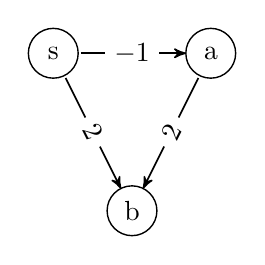
\begin{tikzpicture}[scale = 1.0, transform shape]
    \Vertex[x=0,y=2]{s}
    \Vertex[x=2,y=2]{a}
    \Vertex[x=1,y=0]{b}
    \tikzstyle{LabelStyle}=[fill=white,sloped]
    \tikzstyle{EdgeStyle}=[post]
    \Edge[label=$-1$](s)(a)
    \Edge[label=$2$](s)(b)
    \Edge[label=$2$](a)(b)
\end{tikzpicture}\\
Wir suchen nach dem kuerzestem Weg von s nach b.\\
\\
Nach Bobs Verfahren waehlen wir also nun ein c, so dass 
$$\forall e \in E.c + w(e) > 0, c \in \mathbb{N}$$ 
,mit E als der Menge aller Kanten aus G, gilt.\\
\\
Ein solches c waere hier beispielsweise c=2. Daraus wuerde dann ueber die veraenderte Gewichtsfunktion
$w'(e) = c + w(e)$, der folgenede veraenderte Graph $G'$  resultieren.\\
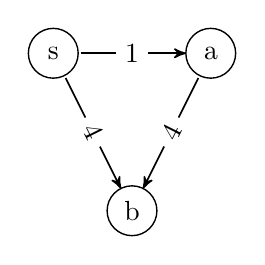
\begin{tikzpicture}[scale = 1.0, transform shape]
    \Vertex[x=0,y=2]{s}
    \Vertex[x=2,y=2]{a}
    \Vertex[x=1,y=0]{b}
    \tikzstyle{LabelStyle}=[fill=white,sloped]
    \tikzstyle{EdgeStyle}=[post]
    \Edge[label=$1$](s)(a)
    \Edge[label=$4$](s)(b)
    \Edge[label=$4$](a)(b)
\end{tikzpicture}\\
\\
Es ist ersichtlich, dass der kuerzeste Weg aus $G$ von s ueber a nach b mit den Kanten $K = \{(s,a),(a,b)\}$ verlaueft.\\
Wuerde man nun aber den Dijkstra-Algorithmus auf $G'$ anwenden waere die kuerzeste Verbindung von s nach b mit den 
Kanten $K' = \{(s,b)\}$. Es gilt $K \neq K'$ damit ist Bobs Verfahren nicht korrekt.\\

\subsubsection \
Bellman-Ford Algorithmus:\\
$d_i$ steht je fuer den i-ten durchlauf.\\
\\
\begin{tabular}{|l|l|l|l|l|l|}
    \hline
    $d_i$&  s&  a&  b&  c&  d\\
    \hline
    $d_0$&  0&\ue&\ue&\ue&\ue\\
    $d_1$&  0&  5&  4&  8&\ue\\
    $d_2$&  0&  2&  4&  8&  3\\
    $d_3$&  0&  2&  4&  8&  0\\
    $d_4$&  0&  2&  4&  6&  0\\
    \hline
\end{tabular}\\
\\
\\
Negative Zyklen:\\
ein Graph enthaelt beispielsweise dann einen negativen Zyklus, wenn sich nach $n = |V| -1$ Iterationen noch
ein Wert in M veraendert.\\
\\
\begin{tabular}{|l|l|l|l|l|l|}
    \hline
    $d_i$&  s&  a&  b&  c&  d\\
    \hline
    $d_4$&  0&  2&  4&  6&  0\\
    $d_5$&  0&  2&  3&  6&  0\\
    \hline
\end{tabular}\\
\\
Aufgrund eines Weges ueber die Kanten $\{(a,d),(d,c),(c,b),(b,a)\}$ veraendern sich auch nach n Iterationen noch Werte.
Damit existiert ein negativer Zyklus.\\
\newpage

\subsection{Graphalgorithmen}
gegeben:\\
\\
(i) Menge von Schmetterlingen $V$, der typisierten Mengen $A,B$\\
(ii) Ferner definieren wir eine Menge $T \subseteq V \times V$ von Tupeln von Schmetterlingen,\\
\tab die der selben typisierten Menge entstammen.\\
(iii) Teilmengen $E \subseteq V, F \subseteq V$ mit den Regeln:\\
\tab 1. $(u,v) \in E \Rightarrow (u, v) \in T$\\
\tab 2. $(u,v) \in F \Rightarrow (u, v) \not \in T$\\
\tab 3. $\forall (u,v) \in V \times V .
    ((u, v) \not \in E \land (u, v) \not \in F) \lor ((u,v) \in E \Leftrightarrow (u,v) \not \in F)$\\ 
\\
\subsubsection \
Ziel des Algorithmus soll sein, auszugeben, ob die Regeln aus (iii) auf Mengen V, E, F gelten.\\
Fuer eine wahre Ausgabe muss gewaehrleistet sein, dass:\\
\tab alle Schmetterlingpaare aus E den selben Typ haben. (iii) 1.\\
\tab alle Schmetterlingpaare aus F nicht den selben Typ haben. (iii) 2.\\
\tab Schmetterlingpaare duerfen in keiner beider Mengen sein, aber nicht in beiden (iii) 3.\\
Nach (iii) 3. reicht es Paare aus E und F zu betrachten.\\
\\
Wir nehmen an, das die Knoten alle als ids, bzw. als int Wert / ganzahlige Zahl zur Verfuegung stehen und man deshalb 
Arrays anhand von ihnen befuellen kann. Weiter nehmen wir an, dass die Methode type(x) den Typen des Knoten x in 
$O(1)$ ausgibt. Der Typ sei mit anderen Typen vergleichbar.\\
Zu Beginn initialisieren wir einen Array dessen Laenge gleich der Anzahl von Knoten des Graphen ist. In diesen Array
wird gespeichert, ob ein Knoten markiert ist oder nicht. Zu Beginn sind alle Knoten unmarkiert.
Zunaechst wird durch E gierig durchgelaufen und geguckt, ob das jeweilige Paar vom gleichen Typen ist.
Ist dies der Fall, so wird jeder Knoten des Paares makiert um zu signalisieren, dass er in E enthalten ist.\\
Danach wird durch F gierig durchgelaufen und geguckt, ob das jeweilige Paar nicht vom gleichen typen ist und nicht beide
Knoten des Paares markiert wurden, bzw. in E enthalten sind.\\
\\
KONSISTENT(V, E, F):\\
1 \tab colors \lA new Array[1...$|V|$]\\
2 \tab for i \lA 1 to $|V|$ do\\
3 \tab \tab colors[i] \lA white\\
4 \tab for each $(s_0, s_1) \in E$ do\\
5 \tab \tab if type($s_0$) = type($s_1$) then\\
6 \tab \tab \tab colors[$s_0$] \lA black\\
7 \tab \tab \tab colors[$s_1$] \lA black\\
8 \tab \tab else\\
9 \tab \tab \tab return False\\
10\tab for each $(s_0, s_1) \in F$ do\\
11\tab \tab if (colors[$s_0$] = black and colors[$s_1$] = black) or (type($s_0$) = type($s_1$)) then\\
12\tab \tab \tab return False\\
13\tab return True\\
\\
\subsubsection \
Es folgen die Operationen je nach Zeile fuer die O-Notation:\\
\begin{tabular}{ll}
    1     &$\in O(1)$\\
    2-3   &$\in O(1 + |V|) = O(|V|)$\\
    4-9   &$\in O(1 + 3 * |E|) = O(|E|)$\\
    10-12 &$\in O(1 + 2 * |F|) = O(|F|)$\\
    13    &$\in O(1)$\\
\end{tabular}\\
Die Zeilen 2-3, 4-9, 10-12 laufen in $O(|V|)$, $O(|E|)$ und  $O(|F|)$ da fuer sie jeweils die Mengen einmal gierig 
durchgegangen werden muesen.\\
Die Zeilen 1, 13 sind nicht an Schleifen gebunden und in Konstanter Laufzeit.\\
Fuer die gesamte Laufzeit in O-Notation ergibt sich:\\
$O(1) + O(|V|) + O(|E|) + O(|F|) = O(1 + |V| + |E| + |F|) = O(|V| + |E| + |F|)$\\
\\
Damit liegt unserer Algorithmus in der gewuenschten Laufzeit $O(|V| + |E| + |F|)$.\\
\subsubsection \
Wie bereits erwaehnt muessen folgende Regeln gelten:\\
\tab (1) alle Schmetterlingpaare aus E den selben Typ haben.\\
\tab (2) alle Schmetterlingpaare aus F nicht den selben Typ haben.\\
\tab (3) Schmetterlingpaare duerfen in keiner beider Mengen sein, aber nicht in beiden.\\
\\
Wir nehmen an ein Paar $(s_0, s_1)$ existiert, fuer dass eine der 3 Regeln, nach dem Ablauf unseres Algorithmus und einer
Ausgabe True oder False, nicht gilt.\\
Wir betrachten jede moegliche Verletzung einer Regel einzelnt.\\
\\
\\
I) Es gilt nicht: (1) alle Schmetterlingpaare aus E den selben Typ haben.\\
In diesem Fall sei also $(s_0, s_1)$ in E und nicht vom selben Typ und es wird True ausgegeben.\\
Dies steht im Widerspruch zu den Zeilen 8-9, die fuer den Fall, dass ein Paar aus E nicht den selben Typ hat direkt 
False ausgeben.\\
\\
II) Es gilt nicht: (2) alle Schmetterlingpaare aus F nicht den selben Typ haben.\\
In diesem Fall sei also $(s_0, s_1)$ in F und vom selben Typ und es wird True ausgegeben.\\
Dies steht im Widerspruch zu den Zeilen 11-12, die fuer den Fall, dass ein Paar aus F den selben Typ hat direkt 
False ausgeben.\\
\\
III) Es gilt nicht: (3) Schmetterlingpaare duerfen in keiner beider Mengen sein, aber nicht in beiden\\
In diesem Fall sei also $(s_0, s_1)$ in E und F und es wird True ausgegeben.\\
Dies steht im Widerspruch zu den Zeilen 5-7 und 11-12, die dafuer zustandig sind alle Schmetterlinge in E zu makieren und
nachdem alle Schmetterlinge aus E makiert wurden in F ueberpruefen, ob beie Schmetterlinge des Paares makiert wurden. Nur
dann waere auch das Paar in E. In diesem Fall wird direkt False ausgegeben.\\
\\
Da Keiner der Faelle moeglich ist, gilt die Annahme nicht und durch Kontraposition wurde gezeigt, dass der Algorithmus
korrekte Ausgaben gibt.\\
\newpage

\subsection{Bonus: Dynamische Programmierung}
\subsubsection \
Das Probelem, der Aufgabe ist die Referenz auf die i-Position aufrecht zu erhalten. Es ist moeglich dass bis zum 
Block $b_{i,j}$ es zweite gleich grosse minimale Strafen gibt, deren i-Differenz groesser 2 ist.\\
Im darauf folgenden j' = j+1 muessen dann alle i-Position beruecksichtigt werden, die eine optimale Strafe ausgeben 
koennten.\\
Damit die Referenz auf die i-Position(en) aufrecht zu erhalten fuellen wir auch noch das Feld pos(i,j), dass fuer jedes
i, j eine Liste mit den i-Positionen enthaelt.\\
\\
E = \begin{cases}

\end{cases}
\subsubsection \
RUN(S):\\
\tab E \lA new Array[0...length(S)][0...lengthS[0]]\\
\tab pos \lA new Array[1...length(S)][1...lengthS[0]]\\
\tab for i \lA 0 to length(E) do\\
\tab \tab E[i][0] \lA \ue\\
\tab for j \lA 1 to length(E[0]) do\\
\tab \tab E[0][j] \lA 0\\
\tab for j \lA 1 to length(E) do\\
\tab \tab E[1][j] \lA E[1][j-1] + S[1][j]\\
\tab \tab pos[1][j] \lA 1\\
\tab tmp1 \lA \ue\\
\tab tmp2 \lA 0\\

\tab for i \lA 2 to length(E) do\\
\tab \tab for j \lA 1 to length(E[0]) do\\
\tab \tab \tab for each $p \in pos[i][j-1]$
\tab \tab \tab \tab val1 \lA S[p][j] + E[i][j-1]\\
\tab \tab \tab \tab val2 \lA S[p][j] + E[i-1][j-1]\\
\tab \tab \tab \tab val3 \lA S[p-1][j] + E[i][j-1]\\
\tab \tab \tab \tab val4 \lA S[p-1][j] + E[i-1][j-1]\\
\tab \tab \tab \tab tmp1 \lA $min\{val1, val2, val3, val4\}$\\
\tab \tab \tab \tab if tmp1 = $min\{val1, val2\}$ then\\
\tab \tab \tab \tab \tab tmp2 += 1
\tab \tab \tab \tab else
\tab \tab \tab \tab \tab tmp2 = 0




\tab result \lA \ue\\
\tab for i \lA 1 to length(E) do\\
\tab \tab result \lA $min\{result, E[i][length(E[0])]\}$\\
\tab return result
\end{document}\\
